%% Based on a TeXnicCenter-Template by Gyorgy SZEIDL.
%%%%%%%%%%%%%%%%%%%%%%%%%%%%%%%%%%%%%%%%%%%%%%%%%%%%%%%%%%%%%

%------------------------------------------------------------
%
\documentclass{article}%
%Options -- Point size:  10pt (default), 11pt, 12pt
%        -- Paper size:  letterpaper (default), a4paper, a5paper, b5paper
%                        legalpaper, executivepaper
%        -- Orientation  (portrait is the default)
%                        landscape
%        -- Print size:  oneside (default), twoside
%        -- Quality      final(default), draft
%        -- Title page   notitlepage, titlepage(default)
%        -- Columns      onecolumn(default), twocolumn
%        -- Equation numbering (equation numbers on the right is the default)
%                        leqno
%        -- Displayed equations (centered is the default)
%                        fleqn (equations start at the same distance from the right side)
%        -- Open bibliography style (closed is the default)
%                        openbib
% For instance the command
%           \documentclass[a4paper,12pt,leqno]{article}
% ensures that the paper size is a4, the fonts are typeset at the size 12p
% and the equation numbers are on the left side
%
\usepackage{amsmath}%
\usepackage{amsfonts}%
\usepackage{amssymb}%
\usepackage{graphicx}
%-------------------------------------------
\newtheorem{theorem}{Theorem}
\newtheorem{acknowledgement}[theorem]{Acknowledgement}
\newtheorem{algorithm}[theorem]{Algorithm}
\newtheorem{axiom}[theorem]{Axiom}
\newtheorem{case}[theorem]{Case}
\newtheorem{claim}[theorem]{Claim}
\newtheorem{conclusion}[theorem]{Conclusion}
\newtheorem{condition}[theorem]{Condition}
\newtheorem{conjecture}[theorem]{Conjecture}
\newtheorem{corollary}[theorem]{Corollary}
\newtheorem{criterion}[theorem]{Criterion}
\newtheorem{definition}[theorem]{Definition}
\newtheorem{example}[theorem]{Example}
\newtheorem{exercise}[theorem]{Exercise}
\newtheorem{lemma}[theorem]{Lemma}
\newtheorem{notation}[theorem]{Notation}
\newtheorem{problem}[theorem]{Problem}
\newtheorem{proposition}[theorem]{Proposition}
\newtheorem{remark}[theorem]{Remark}
\newtheorem{solution}[theorem]{Solution}
\newtheorem{summary}[theorem]{Summary}
\newenvironment{proof}[1][Proof]{\textbf{#1.} }{\ \rule{0.5em}{0.5em}}

\begin{document}

\begin{flushleft}
\textbf{Course:} CSC520, Introduction to Artificial Intelligence\\
\textbf{Homework 2}\\
\textbf{Student: Xusheng Xiao} \\
\textbf{Unity ID: xxiao2} \\
\textbf{Email: xxiao2@ncsu.edu}
\end{flushleft}

\noindent{\hrulefill}

\bigskip

\begin{enumerate}
	\item \textbf{ (34 points) Consider the following English sentences.:}
	\begin{enumerate}
	\item John is a lawyer.
    \item Lawyers are rich.
    \item Rich people have big houses.
    \item Big houses are a lot of work to maintain.
    \item John has a house.
	\end{enumerate}
     
    Answer the following questions:
     \begin{enumerate}
	\item (10 points) Convert the sentences into first order predicate logic. Use the following lexicon: \\
	Functions: $houseof(X)$ -- the house of $X$ \\
	Predicates: $lawyer(X)$ -- $X$ is a lawyer\\
            $rich(X)$ -- $X$ is rich \\
            $big(X)$ -- $X$ is big \\
            $lotofwork(X)$ -- $X$ is a lot of work \\
            $house(X, Y)$ -- the owner of house $X$ is $ Y$\\
        \begin{enumerate}
		\item $ lawyer(john) $
		\item $ \forall X (lawyer(X) \Rightarrow rich(X)) $
		\item $ \forall X (rich(X) \Rightarrow house(houseof(X)) \wedge big(houseof(X)) ) $
		\item $ \forall X (big(houseof(X)) \Rightarrow lotofwork(houseof(X))) $
		\item $ house(houseof(john)) $
		\end{enumerate} 
    \item (12 points) Convert the logic statements into CNF.
    	\begin{enumerate}
		\item $ lawyer(john) $
		\item $ \neg lawyer(X1) \vee rich(X1) $
		\item $ \neg rich(X2) \vee house(houseof(X2)) $ 
		\item $ \neg rich(X3) \vee big(houseof(X3)) $
		\item $ \neg big(houseof(X4)) \vee lotofwork(houseof(X4)) $
		\item $ house(houseof(john)) $
		\end{enumerate}
	\item (12 points) Using resolution, prove that "John's house is a lot of work to maintain." \\
	Conclusion: $ house(houseof(john)) \wedge lotofwork(houseof(john))$\\
		------------------------------------------------\\
		Negated conclusion:  \\
		1. $ \neg house(houseof(john)) \vee \neg lotofwork(houseof(john))$ \\
		------------------------------------------------\\
		\begin{tabular}{c|p{8cm}|l}
		2. & $ rich(john) $ &  $i + ii \lbrace john / X \rbrace$ \\
		3. & $ house(houseof(john)) $ &  $2+ iii \lbrace john / X2 \rbrace$ \\
		4. &$ big(houseof(john))$& $2 + iv \lbrace john / X2 \rbrace$\\
		5. & $ lotofwork(houseof(john)) $ &$ 4 + v \lbrace john / 4 \rbrace$\\
		6. & $ \neg house(houseof(john)) $ &$ 5 + 1 $\\
		7. & $ \emptyset  $ &$ 3 + 6$\\
		\end{tabular} 
	\end{enumerate}
	
\item \textbf{(24 points) Consider the following English sentences.}

	\begin{itemize}
	\item The College of Engineering is in Daniels Hall and the College of Business is in Nelson Hall.
	\item Computer Science and Civil Engineering are departments in the College of Engineering.
	\item Finance is a department in the College of Business.
	\item Smith is a professor in Computer Science, Jones in Civil Engineering, and Edison in Finance.
	\end{itemize}

Now answer the following questions. Submit the final prolog code.

	\begin{enumerate}
	\item (8 points) Convert the English sentences into a Prolog database. \\
	in(ce,daniel). \\
in(cm,nelson). \\
department(cs,ce). \\
department(civil,ce). \\
department(finance,cm). \\
prof(smith,cs). \\
prof(jones,civil). \\
prof(edison,finance). \\



	\item (4 points) Write Prolog rules for each of the following statements and add the rules into the Prolog database.
		\begin{itemize}
		\item A faculty member of a department is also a faculty member in the corresponding College.\\
		
		prof(F,S) :- department(D,S),prof(F,D). \\
		\item The location of the department in the same as the location of corresponding College. \\
		
		in(D,L) :- department(D,C),in(C,L). \\
		\end{itemize}
	\item (4 points) Now, write a query to find the location of Prof. Smith. and show the result. (Hint: the professor will be in same building as his/her department) \\
	
	prof(smith,Dept),in(Dept,Location). \\
	
	Dept = cs,
Location = daniel ;
	
	\item (4 points) Add to the Prolog database a rule with head location(X, Y) that will display the location of a faculty given a query such as location(smith,Where).\\
	
	location(F,L) :- prof(F,D),in(D,L). \\
	\item (4 points) Now write a single query for each of the following questions and show the results.
		\begin{itemize}
		\item Name the faculty in the College of Engineering. \\
		
		prof(Faculty, ce).\\
		
		Faculty = smith ; \\

		Faculty = jones ;
		\item List ALL the occupants of Daniels Hall. \\
		
		in(Occupant, daniel).\\
		
		Occupant = ce ; \\

		Occupant = cs ; \\

		Occupant = civil ; 
		
		\end{itemize}

	\end{enumerate}



\item \textbf{(12 points) Question 3.15 a, b, c, and d from Russell \& Norvig, p. 116. \\
Consider a state space where the start state is number 1 and the successor function for
state n returns two states, numbers 2n and 2n + 1.}
	\begin{enumerate}
	\item Draw the portion of the state space for states 1 to 15.
	
	
\begin{figure}[h]
\centering
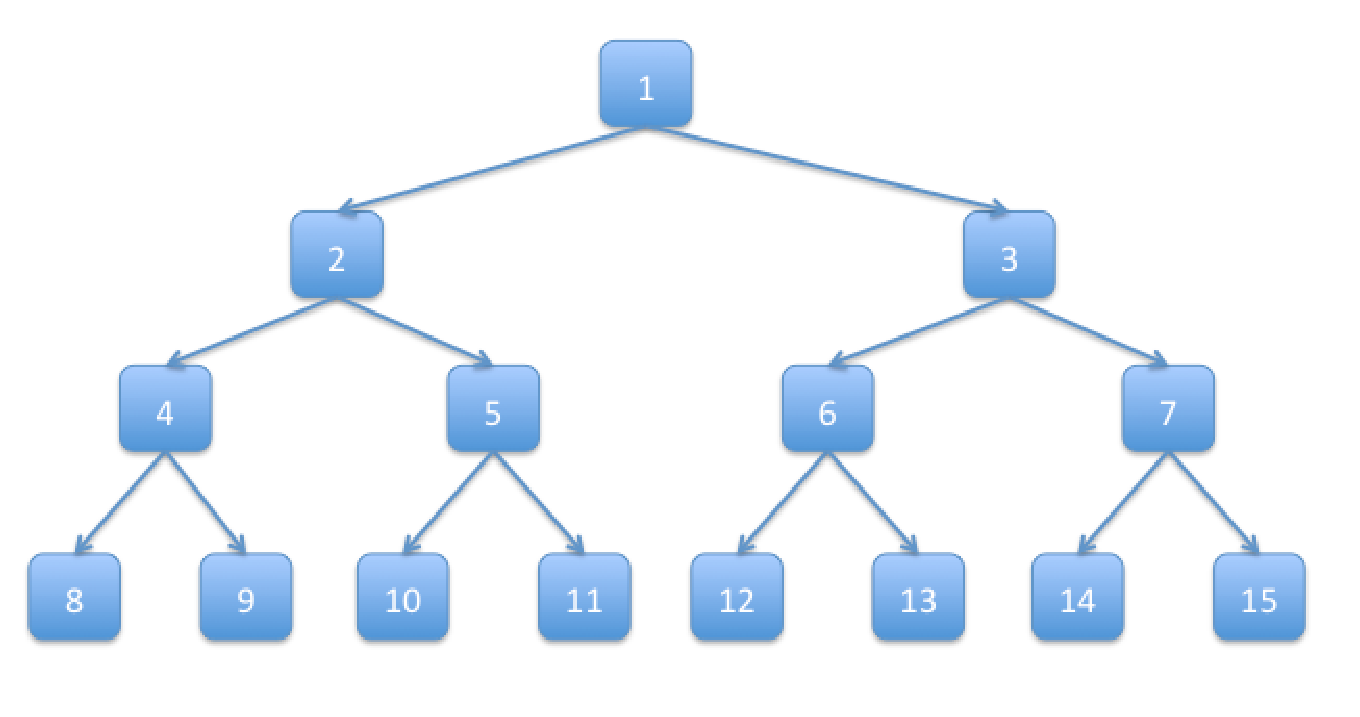
\includegraphics[scale=0.5, clip]{state1-15.eps} 
\vspace*{-2ex}
\end{figure}
	
	\item Suppose the goal state is 11. List the order in which nodes will be visited for breadthfirst
search, depth-limited search with limit 3, and iterative deepening search.

		\begin{itemize}
		\item \textbf{Breadth First Search:} \\
			1,2,3,4,5,6,7,8,9,10,11
		\item \textbf{Depth-limited Search with Limit 3:} \\
		    1,2,4,8,9, 5, 10, 11
		\item \textbf{Iterative Deepening Search:} \\
			1,2,3,4,5,6,7,8,9,10,11
		\end{itemize}
	\item Would bidirectional search be appropriate for this problem? If so, describe in detail
how it would work. \\

	I think bidirectional search is appropriate for this problem. We can apply breadth first search on both start state and goal state. Each direction searches one node at a time. Then the order of nodes visited would be: [1, 2, 3] , [11, 5, 2]. Since it meets at the node 2, the search finds a path.
	
	\item Does the answer to (c) suggest a reformulation of the problem that would allow you to
solve the problem of getting from state 1 to a given goal state with almost no search? \\

	No. Reformulation of the problem sometimes can reduce the search space but cannot eliminate all the search space.
\end{enumerate}
	
\item \textbf{(30 points) Here is a road map of Romania map. (The numbers on the edges indicate the distance between the cities connected, but you don't distances them until Homework 3.).}

\begin{figure}[h]
\centering
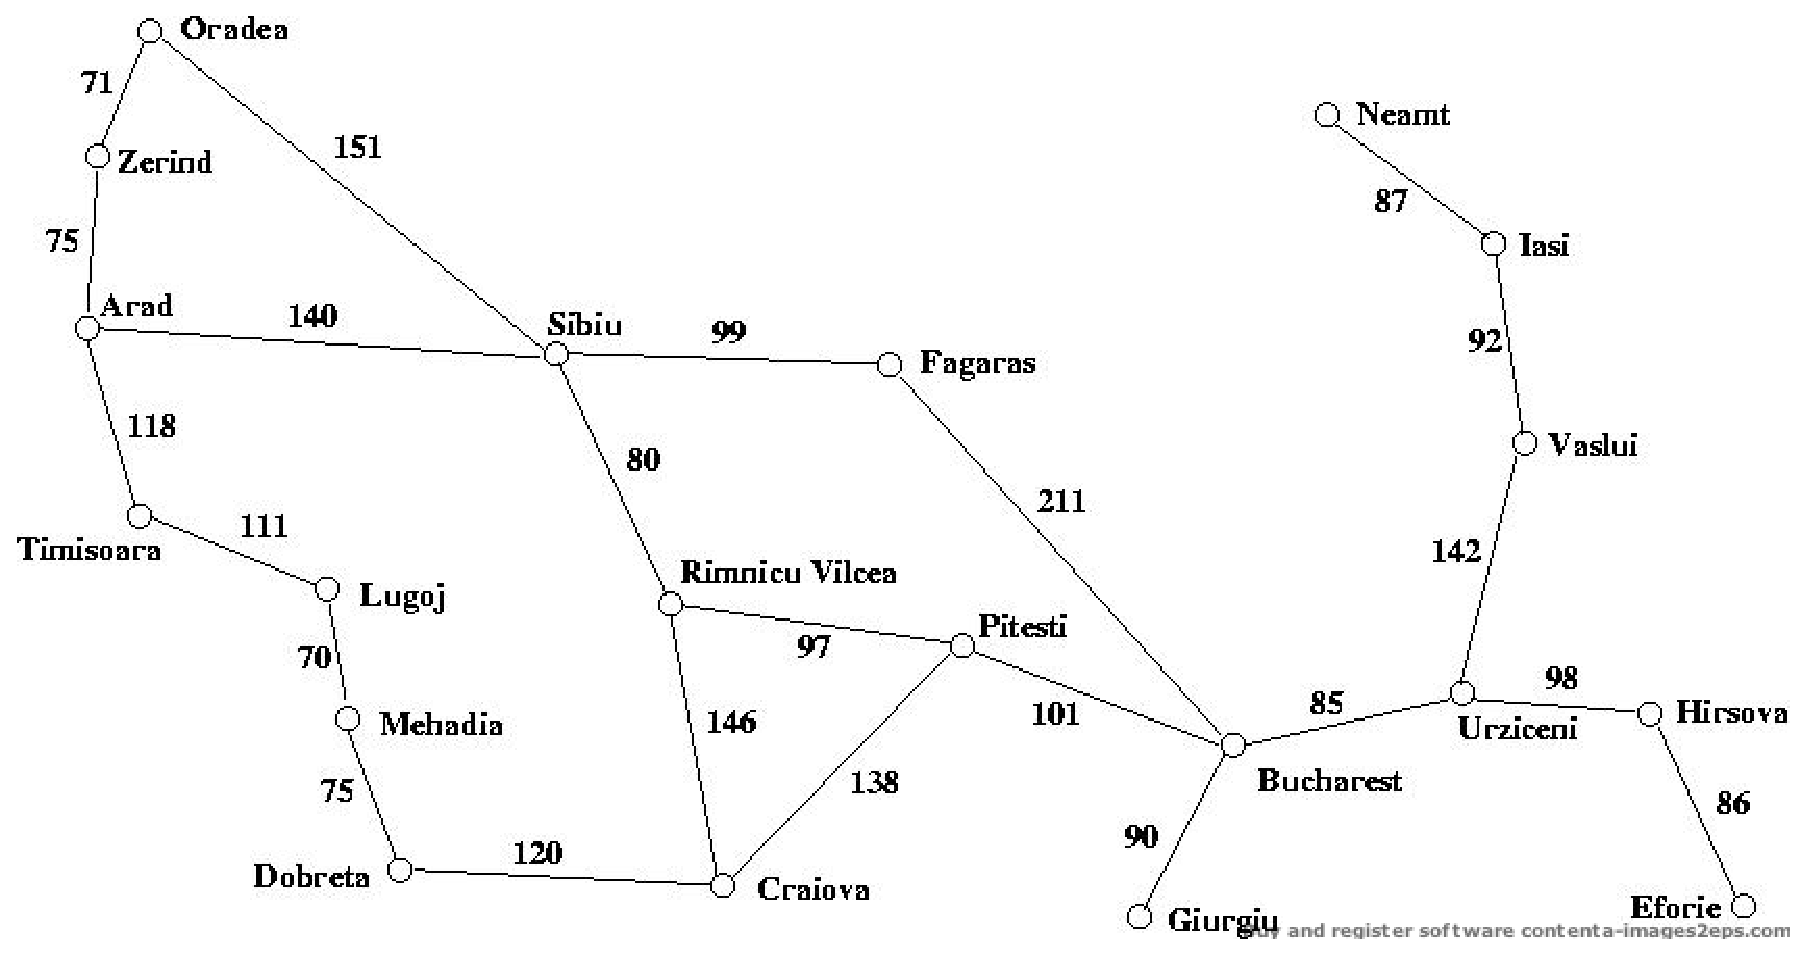
\includegraphics[scale=0.45, clip]{romania.eps} 
\vspace*{-2ex}
\end{figure}

For this assignment, you may use the Prolog source in the webnotes for dfs.pl, bfs2.pl and roads.pl. 

	\begin{enumerate}
	\item (8 points) Consider the path from Arad to Bucharest and the path from Bucharest to Arad. Show the paths returned by DFS and BFS results for each case.
Does either DFS or BFS return a path through the same set of cities for either? Give a reason for this behavior.
		\begin{enumerate}
		\item \textbf{Arad to Bucharest}
			\begin{itemize}
			\item \textbf{DFS}:
				\begin{itemize}
				\item arad timisoara lugoj mehadia dobreta craiova rimnicu\_vilcea pitesti bucharest
				\item arad timisoara lugoj mehadia dobreta craiova rimnicu\_vilcea sibiu fagaras bucharest 
				\item arad timisoara lugoj mehadia dobreta craiova pitesti rimnicu\_vilcea sibiu fagaras bucharest 
				\item arad timisoara lugoj mehadia dobreta craiova pitesti bucharest 
				\item arad sibiu rimnicu\_vilcea craiova pitesti bucharest 
				\item arad sibiu rimnicu\_vilcea pitesti bucharest 
				\item arad sibiu fagaras bucharest 
				\item arad zerind oradea sibiu rimnicu\_vilcea craiova pitesti bucharest 
				\item arad zerind oradea sibiu rimnicu\_vilcea pitesti bucharest 
				\item arad zerind oradea sibiu fagaras bucharest 
				\end{itemize}
			\item \textbf{BFS}:
				\begin{itemize}
				\item arad sibiu fagaras bucharesttrue 
				\item arad sibiu rimnicu\_vilcea pitesti bucharest
				\end{itemize}
			\end{itemize}
		\item \textbf{Bucharest to Arad}
		\begin{itemize}
			\item \textbf{DFS}:
				\begin{itemize}
				\item bucharest pitesti craiova dobreta mehadia lugoj timisoara arad
				\item bucharest pitesti craiova rimnicu\_vilcea sibiu oradea zerind arad
				\item bucharest pitesti craiova rimnicu\_vilcea sibiu arad 
				\item bucharest pitesti rimnicu\_vilcea craiova dobreta mehadia lugoj timisoara arad 
				\item bucharest pitesti rimnicu\_vilcea sibiu oradea zerind arad 
				\item bucharest pitesti rimnicu\_vilcea sibiu arad 
				\item bucharest fagaras sibiu rimnicu\_vilcea craiova dobreta mehadia lugoj timisoara arad 
				\item bucharest fagaras sibiu rimnicu\_vilcea pitesti craiova dobreta mehadia lugoj timisoara arad 
				\item bucharest fagaras sibiu oradea zerind arad 
				\item bucharest fagaras sibiu arad 
				\end{itemize}
			\item \textbf{BFS}:
				\begin{itemize}
				\item bucharest fagaras sibiu aradtrue 
				\end{itemize}
			\end{itemize}
		\end{enumerate}
		
	DFS and BFS do return some paths through same set of cities. In such a undirectional graph, the set of paths found by DFS is the super set of the set of paths found by BFS, since BFS only finds shortest paths in a graph where the weight for each link in the graph is uniform.
	
	\item (6 points) Is there a case where Depth-First performs worse than Breadth-First (in terms of number of cities visited in the path, not the distance) ? If yes, what is it? If not, explain why. \\
	
	Yes. In a path ``arad timisoara lugoj mehadia dobreta craiova rimnicu\_vilcea pitesti bucharest'' found by DFS, BFS found a shorter path ``arad sibiu fagaras bucharesttrue ''.
	
	\item (6 points) Is there a case where Breadth-First performs worse than Depth-First (in terms of number of cities visited in the path, not the distance)? If yes, what is it? If not, explain why. \\
	
	No. Since in such a uniform weight graph, BFS always finds shortest paths.
	
	\item (10 points) For the same graph, perform a hand-execution of Depth-First Iterative Deepening (DFID) with increment and cutoff initialized to 1, starting at Oradea. List the nodes in the order expanded and the state of the data structure for the first five iterations of DFID. Expand the nodes alphabetically and insert them in nondecreasing alphabetical order. Compare this list with Breadth-First Search. (No Prolog is required for the DFID portion of this question.).\\
		\begin{itemize}
		\item \textbf{Limit = 1.} 
			\begin{itemize}
			\item \textbf{expanded nodes:} Oradea
			\item \textbf{data structure:} \\
			$\left[ Oradea , Sibiu \right]$\\
			$\left[ Oradea, Zerind\right]$ 
			\end{itemize}
		\item \textbf{Limit = 2.} 
			\begin{itemize}
			\item \textbf{expanded nodes:} Oradea, Sibiu, Zerind
			\item \textbf{data structure:} \\
			$\left[ Oradea, Sibiu, Arad \right]$\\
			$ \left[ Oradea, Sibiu, Fagaras \right],$ \\ 
			$ \left[ Oradea, Sibiu, Rimnice Vilcea \right]$\\ 
			$\left[ Oradea, Zerind, Arad\right] $ 
			\end{itemize}
		\item \textbf{Limit = 3.} 
			\begin{itemize}
			\item \textbf{expanded nodes:} Oradea, Sibiu, Arad, Fagaras, Rimnice ViLCea, Zerind, Arad, 
			\item \textbf{data structure:} \\
			$\left[ Oradea, Sibiu, Arad,Timisoara \right]$ \\ 
			$\left[ Oradea, Sibiu, Arad,Zerind \right]$ \\ 
			$ \left[ Oradea, Sibiu, Fagaras, Bucharest \right],$ \\ 
			$ \left[ Oradea, Sibiu, Rimnice Vilcea, Craiova \right]$\\
			$\left[ Oradea, Sibiu, Rimnice Vilcea, Pitesti \right]$ \\
			$ \left[ Oradea, Zerind, Arad, Sibiu\right]$ \\ 
			$\left[ Oradea, Zerind, Arad, Timisoara\right] $ 
			\end{itemize}
		\item \textbf{Limit = 4.} 
			\begin{itemize}
			\item \textbf{expanded nodes:} Oradea, Sibiu, Arad, Timisoara,Zerind, Fagaras, Bucharest, Rimnice ViLCea, Craiova, Pitesti, Zerind
			\item \textbf{data structure:} \\
			$\left[ Oradea, Sibiu, Arad,Timisoara, Lugoj \right]$ \\ 
		    $\left[ Oradea, Sibiu, Arad,Zerind \right]$ \\ 
			$ \left[ Oradea, Sibiu, Fagaras, Bucharest, Giurgiu \right]$ \\ 
			$\left[ Oradea, Sibiu, Fagaras, Bucharest, Pitesti \right]$ \\ 
			$ \left[ Oradea, Sibiu, Fagaras, Bucharest, Urziceni \right]$ \\
			$ \left[ Oradea, Sibiu, Rimnice Vilcea, Craiova,Dobreta \right]$ \\ 
			$ \left[ Oradea, Sibiu, Rimnice Vilcea, Craiova,Pitesti \right]$ \\ 
			$\left[ Oradea, Sibiu, Rimnice Vilcea, Pitesti, Bucharest \right] $ \\
			$\left[ Oradea, Sibiu, Rimnice Vilcea, Pitesti, Craiova \right]$ \\
			$ \left[ Oradea, Zerind, Arad, Sibiu, Fagaras\right]$ \\ 
			$\left[ Oradea, Zerind, Arad, Sibiu, Rimnice Vilcea\right]$ \\
			$\left[ Oradea, Zerind, Arad, Timisoara, Lugoj\right] $ 
			\end{itemize}
		\item \textbf{Limit = 5.} 
			\begin{itemize}
			\item \textbf{expanded nodes:} Oradea, Sibiu, Arad, Timisoara,Luogj, Zerind, Fagaras, Bucharest, Giurgiu, Pitesti, Urziceni, Rimnice Vilcea, Craiova, Dobreta, Pitesti, Pitesti, Bucharest, Zerind, Arad, Sibiu, Fagaras, Rimnice Vilcea, Timisoara, Luogj 
			\item \textbf{data structure:} \\
			$\left[ Oradea, Sibiu, Arad,Timisoara, Lugoj, Mehadia \right]$ \\ 
			$\left[ Oradea, Sibiu, Arad,Zerind \right]$ \\ 
			$ \left[ Oradea, Sibiu, Fagaras, Bucharest, Giurgiu \right]$ \\ 
			$\left[ Oradea, Sibiu, Fagaras, Bucharest, Pitesti, Craiova\right]$ \\ 
			$\left[ Oradea, Sibiu, Fagaras, Bucharest, Pitesti, Rimnice Vilcea\right]$ \\ 
			$ \left[ Oradea, Sibiu, Fagaras, Bucharest, Urziceni, Hirsova\right]$ \\
			$ \left[ Oradea, Sibiu, Fagaras, Bucharest, Urziceni, Vaslui\right]$ \\
			$ \left[ Oradea, Sibiu, Rimnice Vilcea, Craiova,Dobreta,Mehadia \right]$ \\ 
			$ \left[ Oradea, Sibiu, Rimnice Vilcea, Craiova,Pitesti, Bucharest \right]$ \\ 
			$\left[ Oradea, Sibiu, Rimnice Vilcea, Pitesti, Bucharest, Giurgiu \right] $ \\
			$\left[ Oradea, Sibiu, Rimnice Vilcea, Pitesti, Bucharest, Urziceni \right] $ \\
			$\left[ Oradea, Sibiu, Rimnice Vilcea, Pitesti, Craiova, Dobreta \right]$ \\
			$ \left[ Oradea, Zerind, Arad, Sibiu, Fagaras, Bucharest\right]$ \\ 
			$\left[ Oradea, Zerind, Arad, Sibiu, Rimnice Vilcea, Craiova\right]$ \\
			$\left[ Oradea, Zerind, Arad, Sibiu, Rimnice Vilcea, Pitesti\right]$ \\
			$\left[ Oradea, Zerind, Arad, Timisoara, Lugoj,Mehadia\right] $ 
			\end{itemize}
		\end{itemize}
	
	\end{enumerate}

\end{enumerate}
\end{document}
